\documentclass[8pt,aspectratio=169]{beamer}
\usetheme{Madrid}
\usecolortheme{seahorse}
\setbeamertemplate{navigation symbols}{}

% Packages
\usepackage{graphicx}
\usepackage{amsmath}
\usepackage{amssymb}
\usepackage{tikz}
\usetikzlibrary{positioning,arrows.meta,shapes}
\usepackage{listings}
\usepackage{xcolor}
\usepackage{colortbl}
\usepackage{arydshln}  % For \hdashline
\usepackage{tcolorbox}

% Math commands
\newcommand{\given}{\mid}

% BSc Pedagogical boxes
\newtcolorbox{checkpoint}[1][]{
    colback=yellow!10!white,
    colframe=yellow!75!black,
    title=\textbf{Checkpoint: #1},
    fonttitle=\bfseries
}

\newtcolorbox{intuition}[1][]{
    colback=purple!5!white,
    colframe=purple!75!black,
    title=\textbf{Intuition: #1},
    fonttitle=\bfseries
}

\newtcolorbox{realworld}[1][]{
    colback=orange!5!white,
    colframe=orange!75!black,
    title=\textbf{Real World: #1},
    fonttitle=\bfseries
}

% Color definitions
\definecolor{mlgreen}{RGB}{46,204,113}
\definecolor{mlblue}{RGB}{52,152,219}
\definecolor{mlorange}{RGB}{230,126,34}

% Title information
\title{Decoding Strategies}
\subtitle{Choosing the Next Word: Accuracy vs Creativity}
\author{}
\date{}

\begin{document}

% Slide 1: Title
\begin{frame}
    \titlepage
    \vfill
    \begin{center}
    {\footnotesize Week 9: Natural Language Processing Course}
    \end{center}
\end{frame}

% Slide 2: Discovery Question
\begin{frame}{Before We Begin: An Experiment}
    \begin{center}
    {\large\bfseries Why Do Some Systems Always Give the Same Answer?}
    \end{center}

    \vspace{0.5em}

    \begin{columns}[T]
        \begin{column}{0.48\textwidth}
            \textbf{Google Autocomplete:}

            \begin{tcolorbox}[colback=blue!5, colframe=blue!50]
            \small
            \texttt{``The weather is\_\_''}

            \vspace{0.3em}
            Always suggests:
            \begin{itemize}
                \item nice today
                \item beautiful
                \item perfect
            \end{itemize}

            \vspace{0.2em}
            \textcolor{red}{\textbf{Same every time!}}
            \end{tcolorbox}

            \vspace{0.5em}

            \textbf{ChatGPT Response:}

            \begin{tcolorbox}[colback=green!5, colframe=green!50]
            \small
            \texttt{``The weather is\_\_''}

            \vspace{0.3em}
            Try 1: ``absolutely gorgeous''\\
            Try 2: ``quite unpredictable''\\
            Try 3: ``exceptionally mild''

            \vspace{0.2em}
            \textcolor{green}{\textbf{Different each time!}}
            \end{tcolorbox}
        \end{column}

        \begin{column}{0.48\textwidth}
            \textbf{The Core Problem:}

            \vspace{0.3em}

            Your language model gives you probabilities:

            \begin{center}
            \begin{tabular}{lr}
            \textbf{Word} & \textbf{Probability} \\
            \hline
            nice & 0.60 \\
            beautiful & 0.20 \\
            perfect & 0.10 \\
            gorgeous & 0.05 \\
            mild & 0.03 \\
            unpredictable & 0.02 \\
            \end{tabular}
            \end{center}

            \vspace{0.5em}

            \begin{checkpoint}[Design Challenge]
            \small
            \textbf{How would YOU pick the next word?}

            \vspace{0.2em}
            Option A: Always pick 0.60? (safe but boring)\\
            Option B: Pick randomly? (creative but risky)\\
            Option C: Something in between?

            \vspace{0.3em}
            \textbf{Key Question:} Can you be 100\% accurate AND 100\% creative?

            \vspace{0.2em}
            Your answer: \_\_\_\_\_\_\_\_\_\_\_\_
            \end{checkpoint}

            \vspace{0.3em}
            {\footnotesize\color{gray}Next slide reveals: This is the DECODING problem!}
        \end{column}
    \end{columns}
\end{frame}

% Slide 3: Six Problems to Solve
\begin{frame}{Six Problems We Need to Solve Today}
    \begin{center}
    {\large\bfseries Each Problem = One Method We'll Learn}
    \end{center}

    \vspace{0.5em}

    \begin{columns}[T]
    \column{0.48\textwidth}

    \begin{tcolorbox}[colback=red!10, colframe=red!50, title=\textbf{Problem 1}]
    \small
    My model keeps repeating itself!

    \vspace{0.2em}
    \textcolor{blue}{\textbf{→ Solution: Beam Search}}
    \end{tcolorbox}

    \vspace{0.3em}

    \begin{tcolorbox}[colback=orange!10, colframe=orange!50, title=\textbf{Problem 2}]
    \small
    Output is always the same (boring!)

    \vspace{0.2em}
    \textcolor{blue}{\textbf{→ Solution: Sampling}}
    \end{tcolorbox}

    \vspace{0.3em}

    \begin{tcolorbox}[colback=yellow!10, colframe=yellow!50, title=\textbf{Problem 3}]
    \small
    Too random, makes no sense!

    \vspace{0.2em}
    \textcolor{blue}{\textbf{→ Solution: Temperature Control}}
    \end{tcolorbox}

    \column{0.48\textwidth}

    \begin{tcolorbox}[colback=green!10, colframe=green!50, title=\textbf{Problem 4}]
    \small
    Sometimes picks very rare/weird words

    \vspace{0.2em}
    \textcolor{blue}{\textbf{→ Solution: Top-k Sampling}}
    \end{tcolorbox}

    \vspace{0.3em}

    \begin{tcolorbox}[colback=cyan!10, colframe=cyan!50, title=\textbf{Problem 5}]
    \small
    Different contexts need different randomness

    \vspace{0.2em}
    \textcolor{blue}{\textbf{→ Solution: Top-p (Nucleus) Sampling}}
    \end{tcolorbox}

    \vspace{0.3em}

    \begin{tcolorbox}[colback=purple!10, colframe=purple!50, title=\textbf{Problem 6}]
    \small
    Which method should I use for my task?

    \vspace{0.2em}
    \textcolor{blue}{\textbf{→ Solution: Task-Specific Guide}}
    \end{tcolorbox}
    \end{columns}

    \vspace{0.5em}

    \begin{center}
    {\footnotesize\color{gray}Today we solve all 6 problems, step by step!}
    \end{center}
\end{frame}

% Slide 4: What We Learned So Far
\begin{frame}{What We've Learned So Far (Weeks 1-8)}
    \begin{center}
    \includegraphics[width=0.95\textwidth]{../figures/weeks_pipeline_to_decoding.pdf}
    \end{center}

    \vspace{-0.3em}

    \begin{tcolorbox}[colback=blue!10]
    \centering
    \textbf{Key Insight:} Every model from Weeks 1-8 produces P(word) for 50,000+ words.\\
    Week 9 is the FINAL STEP: Which word to actually pick?
    \end{tcolorbox}

    \vspace{0.3em}

    \begin{center}
    {\footnotesize From N-grams to Transformers, ALL methods end with a probability distribution.\\
    Decoding is how we convert probabilities → actual text!}
    \end{center}
\end{frame}

% Slide 5: What is Decoding?
\begin{frame}{What Is Decoding?}
    \begin{center}
    {\Large\bfseries The Core Task: Choose the Next Word}
    \end{center}

    \vspace{1em}

    \begin{columns}
    \column{0.48\textwidth}
    \textbf{What Your Model Gives You:}

    \vspace{0.5em}

    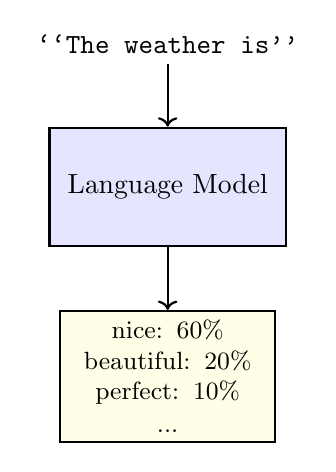
\begin{tikzpicture}[scale=0.9]
        % Neural network box
        \node[draw, thick, rectangle, fill=blue!10, minimum width=3cm, minimum height=1.5cm] (nn) at (0,0) {Language Model};

        % Input
        \node[above=0.8cm of nn] (input) {\texttt{``The weather is''}};
        \draw[->, thick] (input) -- (nn);

        % Output probabilities
        \node[draw, thick, rectangle, fill=yellow!10, below=0.8cm of nn, text width=2.5cm, align=center] (output) {
            \small
            nice: 60\%\\
            beautiful: 20\%\\
            perfect: 10\%\\
            ...
        };
        \draw[->, thick] (nn) -- (output);
    \end{tikzpicture}

    \column{0.48\textwidth}
    \textbf{What You Need to Do:}

    \vspace{0.5em}

    \begin{tcolorbox}[colback=orange!5]
    \textbf{Decoding:} Convert probabilities into actual text
    \end{tcolorbox}

    \vspace{0.5em}

    \textbf{The Trade-off:}

    \begin{center}
    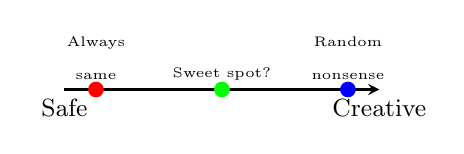
\begin{tikzpicture}[scale=0.8]
        % Spectrum line
        \draw[thick, ->, >=stealth] (0,0) -- (5,0);
        \node[below] at (0,0) {\small Safe};
        \node[below] at (5,0) {\small Creative};

        % Markers
        \node[circle, fill=red, inner sep=2pt] at (0.5,0) {};
        \node[above, text width=1.5cm, align=center] at (0.5,0) {\tiny Always\\same};

        \node[circle, fill=green, inner sep=2pt] at (2.5,0) {};
        \node[above] at (2.5,0) {\tiny Sweet spot?};

        \node[circle, fill=blue, inner sep=2pt] at (4.5,0) {};
        \node[above, text width=1.5cm, align=center] at (4.5,0) {\tiny Random\\nonsense};
    \end{tikzpicture}
    \end{center}

    \vspace{0.5em}

    \textbf{We'll explore:}
    \begin{itemize}
        \item Greedy (always safe)
        \item Beam search (explore paths)
        \item Sampling (add randomness)
        \item How to find YOUR sweet spot
    \end{itemize}
    \end{columns}
\end{frame}

% Slide 6: Greedy Decoding
\begin{frame}{Strategy 1: Greedy Decoding}
    \begin{columns}
    \column{0.48\textwidth}
    \textbf{The Rule:}

    \begin{tcolorbox}[colback=red!10]
    \centering
    \textbf{Always pick the highest probability}
    \end{tcolorbox}

    \vspace{0.5em}

    \textbf{Example:}

    \begin{center}
    \small
    \begin{tabular}{l|c|l}
    \textbf{Step} & \textbf{Probs} & \textbf{Pick} \\
    \hline
    ``The'' & nice:0.6, good:0.3 & nice \\
    ``nice'' & day:0.7, weather:0.2 & day \\
    ``day'' & is:0.5, was:0.3 & is \\
    \end{tabular}
    \end{center}

    \vspace{0.3em}
    Result: ``The nice day is...''

    \vspace{0.5em}

    \textbf{Pros:}
    \begin{itemize}
        \item Fast
        \item Deterministic (same every time)
        \item High probability output
    \end{itemize}

    \column{0.48\textwidth}
    \textbf{The Problem:}

    \begin{tcolorbox}[colback=yellow!20]
    \small
    \textbf{Greedy often gets stuck!}

    \vspace{0.3em}
    Example:\\
    ``The dog likes the dog likes the dog likes...''

    \vspace{0.3em}
    Why? Each step picks ``the'' (0.4) over ``a'' (0.3),\\
    but the FULL sequence ``a cat'' (0.3$\times$0.5=0.15)\\
    beats ``the dog'' (0.4$\times$0.2=0.08)!
    \end{tcolorbox}

    \vspace{0.5em}

    \textbf{Cons:}
    \begin{itemize}
        \item Repetitive
        \item Gets stuck in loops
        \item Misses better sequences
        \item Boring/generic output
    \end{itemize}

    \vspace{0.5em}

    \begin{intuition}[Why Greedy Fails]
    \small
    Locally optimal $\neq$ globally optimal!
    \end{intuition}
    \end{columns}
\end{frame}

% Slide 7: Beam Search Motivation
\begin{frame}{Strategy 2: Beam Search}
    \begin{center}
    {\large\bfseries Idea: Keep Multiple Paths Open}
    \end{center}

    \vspace{0.5em}

    \begin{columns}
    \column{0.48\textwidth}
    \textbf{The Analogy:}

    \begin{tcolorbox}[colback=blue!5]
    \small
    \textbf{GPS Navigation:}

    \vspace{0.3em}
    Greedy: Take fastest road NOW\\
    $\rightarrow$ Might hit traffic later

    \vspace{0.3em}
    Beam: Consider top 3-5 routes\\
    $\rightarrow$ Pick best COMPLETE path
    \end{tcolorbox}

    \vspace{0.5em}

    \textbf{The Rule:}

    \begin{tcolorbox}[colback=green!10]
    \centering
    Keep top-k hypotheses at each step
    \end{tcolorbox}

    \vspace{0.3em}

    \textbf{Beam Size = 3:}
    \begin{itemize}
        \item Track 3 best sequences
        \item Expand each by V words
        \item Keep top 3 of all candidates
        \item Repeat until done
    \end{itemize}

    \column{0.48\textwidth}
    \textbf{Concrete Example (beam=3):}

    \begin{center}
    \small
    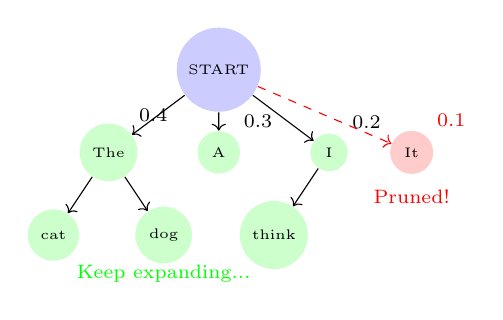
\begin{tikzpicture}[scale=0.7, every node/.style={font=\tiny}]
        % Level 0
        \node[circle, fill=blue!20] (start) at (3,5) {START};

        % Level 1 (keep top 3)
        \node[circle, fill=green!20] (a1) at (1,3.5) {The};
        \node[above right, font=\scriptsize] at (a1.north east) {0.4};
        \node[circle, fill=green!20] (a2) at (3,3.5) {A};
        \node[above right, font=\scriptsize] at (a2.north east) {0.3};
        \node[circle, fill=green!20] (a3) at (5,3.5) {I};
        \node[above right, font=\scriptsize] at (a3.north east) {0.2};
        \node[circle, fill=red!20, dashed] (a4) at (6.5,3.5) {It};
        \node[above right, font=\scriptsize, red] at (a4.north east) {0.1};

        \draw[->] (start) -- (a1);
        \draw[->] (start) -- (a2);
        \draw[->] (start) -- (a3);
        \draw[->, red, dashed] (start) -- (a4);

        % Level 2 (expand top 3, keep top 3)
        \node[circle, fill=green!20] (b1) at (0,2) {cat};
        \node[circle, fill=green!20] (b2) at (2,2) {dog};
        \node[circle, fill=green!20] (b3) at (4,2) {think};

        \draw[->] (a1) -- (b1);
        \draw[->] (a1) -- (b2);
        \draw[->] (a3) -- (b3);

        % Annotations
        \node[red, font=\scriptsize] at (6.5,2.7) {Pruned!};
        \node[green, font=\scriptsize] at (2,1.3) {Keep expanding...};
    \end{tikzpicture}
    \end{center}

    \vspace{0.3em}

    \textbf{Scoring:}

    Score = $\sum \log P(\text{word}_i)$

    \vspace{0.3em}

    Example:\\
    ``The cat'' = $\log(0.4) + \log(0.5) = -0.61$\\
    ``A dog'' = $\log(0.3) + \log(0.4) = -1.22$
    \end{columns}
\end{frame}

% Slide 8: Beam Search Visualization
\begin{frame}{Beam Search: The Full Picture}
    \begin{center}
    \includegraphics[width=0.85\textwidth]{../figures/beam_search_tree.pdf}
    \end{center}

    \vspace{-0.3em}

    \begin{columns}
    \column{0.48\textwidth}
    \begin{tcolorbox}[colback=green!5, colframe=green!50]
    \small
    \textbf{Pros:}
    \begin{itemize}
        \item Better than greedy
        \item Considers context
        \item Good for translation
    \end{itemize}
    \end{tcolorbox}

    \column{0.48\textwidth}
    \begin{tcolorbox}[colback=red!5, colframe=red!50]
    \small
    \textbf{Cons:}
    \begin{itemize}
        \item Still deterministic
        \item Still can be repetitive
        \item Computationally expensive
    \end{itemize}
    \end{tcolorbox}
    \end{columns}
\end{frame}

% Slide 9: Checkpoint 1
\begin{frame}{Checkpoint: Understanding Greedy vs Beam}
    \begin{center}
    {\large\bfseries Test Your Understanding}
    \end{center}

    \vspace{0.5em}

    \begin{columns}
    \column{0.48\textwidth}
    \textbf{Question 1:}

    Why does greedy decoding sometimes produce worse sequences than beam search?

    \begin{enumerate}[A)]
        \item Greedy is slower
        \item Greedy only looks one step ahead
        \item Greedy uses wrong probabilities
        \item Greedy is random
    \end{enumerate}

    \vspace{1em}

    \textbf{Question 2:}

    If beam size = 1, what is beam search equivalent to?

    \begin{enumerate}[A)]
        \item Random sampling
        \item Greedy decoding
        \item Exhaustive search
        \item Top-k sampling
    \end{enumerate}

    \column{0.48\textwidth}
    \textbf{Answer 1:} B

    \begin{tcolorbox}[colback=green!5]
    \small
    Greedy picks best word NOW, ignoring future consequences. Beam search considers multiple paths and picks best FULL sequence.

    \vspace{0.3em}
    Example: ``the dog'' (0.4$\times$0.2) loses to ``a cat'' (0.3$\times$0.5) overall!
    \end{tcolorbox}

    \vspace{0.5em}

    \textbf{Answer 2:} B

    \begin{tcolorbox}[colback=green!5]
    \small
    Beam size = 1 means we only keep 1 hypothesis at each step = greedy decoding!

    \vspace{0.3em}
    Beam search generalizes greedy.
    \end{tcolorbox}
    \end{columns}
\end{frame}

% Slide 10: Sampling Introduction
\begin{frame}{Strategy 3: Sampling - Add Randomness}
    \begin{center}
    {\large\bfseries Problem: Greedy and Beam are TOO Predictable}
    \end{center}

    \vspace{0.5em}

    \begin{columns}
    \column{0.48\textwidth}
    \textbf{Why Randomness?}

    \begin{realworld}[Human Writing]
    \small
    Humans don't always pick the most probable word!

    \vspace{0.3em}
    \textbf{Boring:} ``The weather is nice today''\\
    \textbf{Better:} ``The weather is absolutely gorgeous''

    \vspace{0.3em}
    ``gorgeous'' might have P=0.05, but it's more interesting!
    \end{realworld}

    \vspace{0.5em}

    \textbf{Pure Sampling:}

    \begin{tcolorbox}[colback=blue!10]
    \centering
    Sample from the full probability distribution
    \end{tcolorbox}

    \vspace{0.3em}

    If P(nice)=0.6, P(gorgeous)=0.05:\\
    $\rightarrow$ 60\% chance of ``nice''\\
    $\rightarrow$ 5\% chance of ``gorgeous''

    \column{0.48\textwidth}
    \textbf{Concrete Example:}

    \begin{center}
    \small
    \begin{tabular}{lc}
    \textbf{Word} & \textbf{P} \\
    \hline
    nice & 0.60 \\
    beautiful & 0.20 \\
    perfect & 0.10 \\
    gorgeous & 0.05 \\
    mild & 0.03 \\
    weird & 0.02 \\
    \end{tabular}
    \end{center}

    \vspace{0.5em}

    \textbf{5 samples might give:}
    \begin{enumerate}
        \item nice (highest prob)
        \item nice (again)
        \item beautiful
        \item gorgeous (surprise!)
        \item nice
    \end{enumerate}

    \vspace{0.5em}

    \textbf{Problem:} Sometimes picks ``weird''!
    \end{columns}
\end{frame}

% Slide 11: Temperature
\begin{frame}{Temperature: Control the Randomness}
    \begin{columns}
    \column{0.48\textwidth}
    \textbf{The Formula:}

    \begin{equation*}
    P_T(w_i) = \frac{\exp(z_i / T)}{\sum_j \exp(z_j / T)}
    \end{equation*}

    where $z_i$ = logit, $T$ = temperature

    \vspace{0.5em}

    \textbf{What Temperature Does:}

    \begin{itemize}
        \item $T < 1$: Sharper (more confident)
        \item $T = 1$: Original distribution
        \item $T > 1$: Flatter (more random)
    \end{itemize}

    \vspace{0.5em}

    \begin{tcolorbox}[colback=purple!5]
    \small
    \textbf{Analogy:}

    High temperature = melted ice cream\\
    (everything mixes together, uniform)

    Low temperature = frozen ice cream\\
    (distinct flavors, concentrated)
    \end{tcolorbox}

    \column{0.48\textwidth}
    \textbf{Concrete Example:}

    Original: [0.6, 0.2, 0.1, 0.05, 0.05]

    \vspace{0.3em}

    \begin{center}
    \small
    \begin{tabular}{l|ccccc}
    \textbf{T} & nice & beautiful & perfect & gorgeous & mild \\
    \hline
    0.5 & 0.82 & 0.13 & 0.03 & 0.01 & 0.01 \\
    1.0 & 0.60 & 0.20 & 0.10 & 0.05 & 0.05 \\
    1.5 & 0.45 & 0.25 & 0.15 & 0.08 & 0.07 \\
    2.0 & 0.35 & 0.27 & 0.18 & 0.11 & 0.09 \\
    \end{tabular}
    \end{center}

    \vspace{0.5em}

    \textbf{Recommendations:}
    \begin{itemize}
        \item Factual Q\&A: T=0.1-0.3
        \item Translation: T=0.3-0.7
        \item Dialogue: T=0.7-1.0
        \item Creative writing: T=0.9-1.5
    \end{itemize}
    \end{columns}
\end{frame}

% Slide 12: Temperature Effects Visualization
\begin{frame}{Temperature in Action}
    \begin{center}
    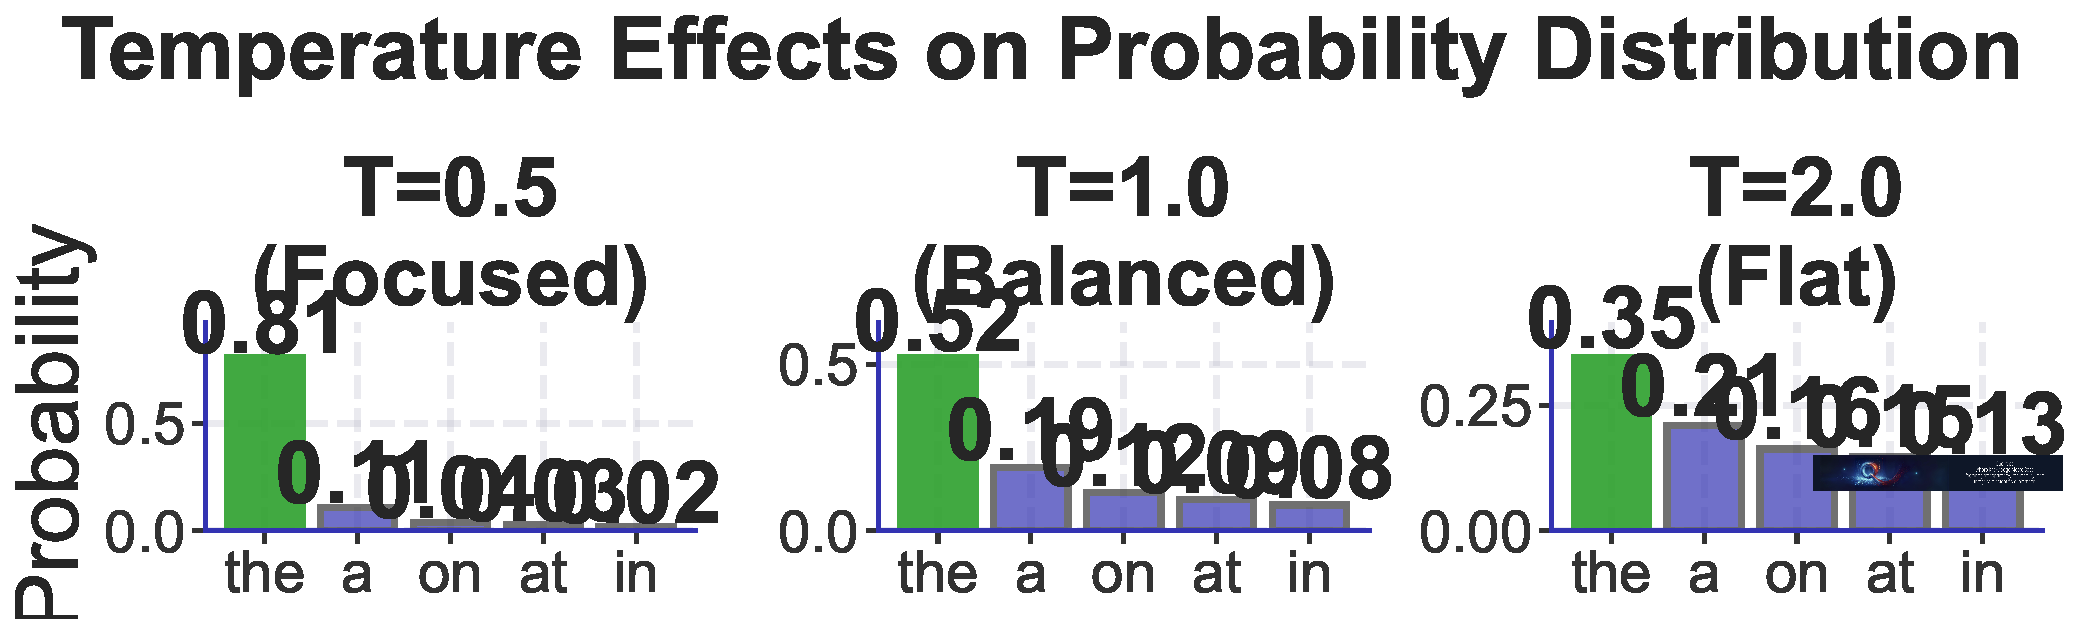
\includegraphics[width=0.95\textwidth]{../figures/temperature_effects.pdf}
    \end{center}

    \vspace{-0.5em}

    \begin{tcolorbox}[colback=yellow!10]
    \centering
    \small
    \textbf{Key Insight:} Temperature lets you control the creativity-accuracy tradeoff!
    \end{tcolorbox}
\end{frame}

% Slide 13: Top-k Sampling
\begin{frame}{Top-k Sampling: Limit the Vocabulary}
    \begin{columns}
    \column{0.48\textwidth}
    \textbf{The Problem with Pure Sampling:}

    \begin{tcolorbox}[colback=red!10]
    \small
    With 50,000 word vocabulary, might sample very unlikely words!

    \vspace{0.3em}
    ``The weather is \textcolor{red}{xylophone}'' (P=0.00001)
    \end{tcolorbox}

    \vspace{0.5em}

    \textbf{The Solution:}

    \begin{tcolorbox}[colback=green!10]
    \centering
    Only sample from top-k most likely words
    \end{tcolorbox}

    \vspace{0.5em}

    \textbf{Example (k=10):}

    \begin{enumerate}
        \item Sort words by probability
        \item Keep only top 10
        \item Renormalize probabilities
        \item Sample from these 10
    \end{enumerate}

    \column{0.48\textwidth}
    \textbf{Concrete Example:}

    Full vocabulary (50,000 words):\\
    nice (0.6), beautiful (0.2), ... xylophone (0.00001)

    \vspace{0.3em}

    \textbf{Top-k=5:}

    \begin{center}
    \small
    \begin{tabular}{lcc}
    \textbf{Word} & \textbf{Original} & \textbf{Renormalized} \\
    \hline
    nice & 0.60 & 0.632 \\
    beautiful & 0.20 & 0.211 \\
    perfect & 0.10 & 0.105 \\
    gorgeous & 0.05 & 0.053 \\
    mild & 0.03 & 0.032 \\
    \hline
    \multicolumn{2}{l}{Others (49,995 words)} & 0.000 \\
    \end{tabular}
    \end{center}

    \vspace{0.5em}

    \textbf{Typical values:}
    \begin{itemize}
        \item k=10: Very focused
        \item k=40: Balanced
        \item k=100: Diverse
    \end{itemize}
    \end{columns}
\end{frame}

% Slide 14: Top-p (Nucleus) Sampling
\begin{frame}{Top-p Sampling: Dynamic Vocabulary}
    \begin{columns}
    \column{0.48\textwidth}
    \textbf{Problem with Top-k:}

    \begin{tcolorbox}[colback=orange!10]
    \small
    Fixed k doesn't adapt to distribution!

    \vspace{0.3em}
    Flat distribution: k=40 might be too few\\
    Peaked distribution: k=40 might include junk
    \end{tcolorbox}

    \vspace{0.5em}

    \textbf{Top-p Solution:}

    \begin{tcolorbox}[colback=blue!10]
    \centering
    Keep smallest set with cumulative probability $\geq$ p
    \end{tcolorbox}

    \vspace{0.5em}

    \textbf{Algorithm:}
    \begin{enumerate}
        \item Sort by probability
        \item Add words until cumsum $\geq$ p
        \item Sample from this ``nucleus''
    \end{enumerate}

    \column{0.48\textwidth}
    \textbf{Example (p=0.9):}

    \begin{center}
    \small
    \begin{tabular}{lccc}
    \textbf{Word} & \textbf{P} & \textbf{Cumsum} & \textbf{Include?} \\
    \hline
    nice & 0.60 & 0.60 & \checkmark \\
    beautiful & 0.20 & 0.80 & \checkmark \\
    perfect & 0.10 & 0.90 & \checkmark \\
    \hdashline
    gorgeous & 0.05 & 0.95 & $\times$ \\
    mild & 0.03 & 0.98 & $\times$ \\
    weird & 0.02 & 1.00 & $\times$ \\
    \end{tabular}
    \end{center}

    Keep 3 words (dynamic!)

    \vspace{0.5em}

    \textbf{Advantages:}
    \begin{itemize}
        \item Adapts to distribution shape
        \item Prevents sampling tail
        \item More robust than top-k
    \end{itemize}

    \vspace{0.5em}

    \textbf{Typical values:}
    p=0.9 or p=0.95
    \end{columns}
\end{frame}

% Slide 15: Top-k vs Top-p Visualization
\begin{frame}{Top-k vs Top-p: Side by Side}
    \begin{center}
    \includegraphics[width=0.9\textwidth]{../figures/sampling_strategies.pdf}
    \end{center}

    \vspace{-0.3em}

    \colorbox{purple!10}{\parbox{0.9\textwidth}{
    \centering\small
    \textbf{Key Difference:} Top-k is fixed, Top-p adapts to distribution shape
    }}
\end{frame}

% Slide 16: The Decoding Landscape
\begin{frame}{The Complete Decoding Landscape}
    \begin{center}
    \includegraphics[width=0.75\textwidth]{../figures/decoding_landscape.pdf}
    \end{center}

    \vspace{-0.5em}

    \begin{tcolorbox}[colback=green!5]
    \centering
    \small
    \textbf{Finding Your Sweet Spot:} Balance safety and creativity for your task
    \end{tcolorbox}
\end{frame}

% Slide 17: Checkpoint 2
\begin{frame}{Checkpoint: Understanding Sampling Methods}
    \begin{center}
    {\large\bfseries Test Your Understanding}
    \end{center}

    \vspace{0.5em}

    \begin{columns}
    \column{0.48\textwidth}
    \textbf{Question 1:}

    What does temperature=0.1 do?

    \begin{enumerate}[A)]
        \item Makes distribution flatter
        \item Makes distribution sharper
        \item Removes low-prob words
        \item Adds randomness
    \end{enumerate}

    \vspace{1em}

    \textbf{Question 2:}

    Distribution: [0.7, 0.15, 0.10, 0.03, 0.02]\\
    With p=0.9, how many words in nucleus?

    \begin{enumerate}[A)]
        \item 1
        \item 2
        \item 3
        \item 5
    \end{enumerate}

    \column{0.48\textwidth}
    \textbf{Answer 1:} B

    \begin{tcolorbox}[colback=green!5]
    \small
    Low temperature (T$<$1) makes the distribution SHARPER = more confident = less random.

    \vspace{0.3em}
    Example: [0.6, 0.2, 0.2] becomes [0.8, 0.1, 0.1]
    \end{tcolorbox}

    \vspace{0.5em}

    \textbf{Answer 2:} C (3 words)

    \begin{tcolorbox}[colback=green!5]
    \small
    Cumulative sum:\\
    0.7 (word 1)\\
    0.85 (word 2)\\
    0.95 (word 3) $\leftarrow$ exceeds 0.9!

    \vspace{0.3em}
    Stop here, use 3 words.
    \end{tcolorbox}
    \end{columns}
\end{frame}

% Slide 18: Combining Methods
\begin{frame}{Combining Decoding Strategies}
    \begin{center}
    {\large\bfseries You Can Use Multiple Techniques Together!}
    \end{center}

    \vspace{0.5em}

    \begin{columns}
    \column{0.48\textwidth}
    \textbf{Common Combinations:}

    \begin{tcolorbox}[colback=blue!5]
    \textbf{Temperature + Top-p}

    \vspace{0.3em}
    \begin{enumerate}
        \item Apply temperature scaling
        \item Filter with top-p
        \item Sample from nucleus
    \end{enumerate}

    \vspace{0.3em}
    Example: T=0.8, p=0.95
    \end{tcolorbox}

    \vspace{0.5em}

    \begin{tcolorbox}[colback=green!5]
    \textbf{Beam + Sampling}

    \vspace{0.3em}
    Beam search, but sample within beam instead of greedy expansion

    \vspace{0.3em}
    Gets diversity + good paths
    \end{tcolorbox}

    \column{0.48\textwidth}
    \textbf{Additional Tricks:}

    \begin{itemize}
        \item \textbf{Repetition penalty:} Reduce prob of recently used words
        \item \textbf{Length normalization:} Don't favor short sequences
        \item \textbf{Min-p:} Absolute minimum threshold
        \item \textbf{Typical sampling:} Sample based on entropy
    \end{itemize}

    \vspace{0.5em}

    \begin{realworld}[ChatGPT Settings]
    \small
    ChatGPT uses temperature + top-p:

    \vspace{0.3em}
    \textbf{Default:} T=0.7, p=0.95\\
    \textbf{Creative mode:} T=0.9\\
    \textbf{Precise mode:} T=0.3
    \end{realworld}
    \end{columns}
\end{frame}

% Slide 19: Performance Metrics
\begin{frame}{Evaluating Decoding Quality}
    \begin{center}
    \includegraphics[width=0.95\textwidth]{../figures/decoding_quality_metrics.pdf}
    \end{center}

    \vspace{-0.5em}

    \colorbox{orange!10}{\parbox{0.9\textwidth}{
    \centering\small
    \textbf{No single best method!} Different tasks need different strategies.
    }}
\end{frame}

% Slide 20: Task-Specific Guide
\begin{frame}{Which Method for Which Task?}
    \begin{center}
    \includegraphics[width=0.7\textwidth]{../figures/decoding_selection_guide.pdf}
    \end{center}
\end{frame}

% Slide 21: Factual QA Example
\begin{frame}{Example 1: Factual Question Answering}
    \begin{columns}
    \column{0.48\textwidth}
    \textbf{Task:} Answer: ``What is the capital of France?''

    \vspace{0.5em}

    \textbf{Priority:} Accuracy $>$ Creativity

    \vspace{0.5em}

    \begin{tcolorbox}[colback=green!10]
    \textbf{Best Strategy:}

    \vspace{0.3em}
    Greedy or Beam-3

    \vspace{0.3em}
    Temperature = 0.1-0.3
    \end{tcolorbox}

    \vspace{0.5em}

    \textbf{Results:}

    \begin{tabular}{l|l}
    \textbf{Method} & \textbf{Output} \\
    \hline
    Greedy & ``Paris'' \\
    T=0.8 & ``Paris, the city of lights'' \\
    T=1.5 & ``Lyon is also nice'' \\
    \end{tabular}

    \column{0.48\textwidth}
    \textbf{Why Greedy Wins:}

    \begin{itemize}
        \item Only ONE correct answer
        \item Creativity adds errors
        \item Speed matters
        \item Consistency important
    \end{itemize}

    \vspace{0.5em}

    \begin{realworld}[Search Engines]
    \small
    Google uses greedy-like decoding for autocomplete:

    \vspace{0.3em}
    \begin{itemize}
        \item Must be accurate
        \item Must be fast
        \item Consistency builds trust
        \item Users want predictability
    \end{itemize}
    \end{realworld}

    \vspace{0.5em}

    \textbf{Metrics:}

    Accuracy: 95\% (greedy) vs 70\% (T=1.5)
    \end{columns}
\end{frame}

% Slide 22: Creative Writing Example
\begin{frame}{Example 2: Creative Story Writing}
    \begin{columns}
    \column{0.48\textwidth}
    \textbf{Task:} Continue: ``Once upon a time...''

    \vspace{0.5em}

    \textbf{Priority:} Creativity $>$ Accuracy

    \vspace{0.5em}

    \begin{tcolorbox}[colback=purple!10]
    \textbf{Best Strategy:}

    \vspace{0.3em}
    Top-k=50 or Top-p=0.95

    \vspace{0.3em}
    Temperature = 0.9-1.2
    \end{tcolorbox}

    \vspace{0.5em}

    \textbf{Comparison:}

    \small
    \textbf{Greedy:}\\
    ``Once upon a time there was a beautiful princess...''

    \vspace{0.3em}

    \textbf{T=1.0, p=0.95:}\\
    ``Once upon a time, beneath an ancient oak, a curious raven discovered...''

    \column{0.48\textwidth}
    \textbf{Why Sampling Wins:}

    \begin{itemize}
        \item Many valid continuations
        \item Repetition is boring
        \item Readers want surprise
        \item No ``ground truth''
    \end{itemize}

    \vspace{0.5em}

    \begin{realworld}[NovelAI]
    \small
    AI writing assistants use:

    \vspace{0.3em}
    \begin{itemize}
        \item Temperature: 0.8-1.2
        \item Top-p: 0.9-0.95
        \item Repetition penalty: 1.1
        \item Users can adjust!
    \end{itemize}
    \end{realworld}

    \vspace{0.5em}

    \textbf{Human Preference:}

    75\% prefer sampling over greedy for stories
    \end{columns}
\end{frame}

% Slide 23: Code Generation Example
\begin{frame}[fragile]{Example 3: Code Generation}
    \begin{columns}
    \column{0.48\textwidth}
    \textbf{Task:} Complete: \texttt{def factorial(n):}

    \vspace{0.5em}

    \textbf{Priority:} Correctness + Some diversity

    \vspace{0.5em}

    \begin{tcolorbox}[colback=blue!10]
    \textbf{Best Strategy:}

    \vspace{0.3em}
    Beam search (size=5)

    \vspace{0.3em}
    Temperature = 0.2-0.5
    \end{tcolorbox}

    \vspace{0.5em}

    \textbf{Why Beam:}

    \begin{itemize}
        \item Syntax must be correct
        \item But multiple valid solutions
        \item Beam finds different approaches
        \item Pick best with tests
    \end{itemize}

    \column{0.48\textwidth}
    \textbf{Results:}

    \small
    \textbf{Greedy (always same):}
\begin{lstlisting}[language=Python, basicstyle=\tiny]
if n == 0:
    return 1
return n * factorial(n-1)
\end{lstlisting}

    \vspace{0.3em}

    \textbf{Beam (multiple options):}
\begin{lstlisting}[language=Python, basicstyle=\tiny]
# Option 1: Recursive
return 1 if n==0 else n*factorial(n-1)

# Option 2: Iterative
result = 1
for i in range(1, n+1):
    result *= i
return result
\end{lstlisting}

    \vspace{0.5em}

    \textbf{Metrics:}

    Pass rate: Beam-5 (85\%) $>$ Greedy (78\%)
    \end{columns}
\end{frame}

% Slide 24: Hyperparameter Tuning
\begin{frame}{Practical Tips: Tuning Your Parameters}
    \begin{columns}
    \column{0.48\textwidth}
    \textbf{Start Conservative:}

    \begin{enumerate}
        \item Begin with T=0.7, p=0.9
        \item Generate 10 samples
        \item Evaluate quality
        \item Adjust based on problems
    \end{enumerate}

    \vspace{0.5em}

    \begin{tcolorbox}[colback=red!10]
    \textbf{Problem: Too repetitive?}

    \vspace{0.3em}
    $\rightarrow$ Increase T (try 1.0)\\
    $\rightarrow$ Increase p (try 0.95)\\
    $\rightarrow$ Add repetition penalty
    \end{tcolorbox}

    \vspace{0.5em}

    \begin{tcolorbox}[colback=blue!10]
    \textbf{Problem: Too random/nonsensical?}

    \vspace{0.3em}
    $\rightarrow$ Decrease T (try 0.5)\\
    $\rightarrow$ Decrease p (try 0.85)\\
    $\rightarrow$ Try beam search
    \end{tcolorbox}

    \column{0.48\textwidth}
    \textbf{Grid Search Strategy:}

    \begin{center}
    \small
    \begin{tabular}{cc|c}
    \textbf{T} & \textbf{p} & \textbf{Quality} \\
    \hline
    0.5 & 0.9 & High acc, boring \\
    0.7 & 0.9 & Balanced \\
    1.0 & 0.9 & Creative \\
    0.7 & 0.95 & More diverse \\
    1.2 & 0.95 & Very creative \\
    \end{tabular}
    \end{center}

    \vspace{0.5em}

    \textbf{Evaluation Metrics:}

    \begin{itemize}
        \item \textbf{Distinct-n:} Unique n-grams (diversity)
        \item \textbf{Perplexity:} Model confidence
        \item \textbf{Repetition rate:} n-gram overlap
        \item \textbf{Human eval:} Ultimate test
    \end{itemize}

    \vspace{0.5em}

    \begin{intuition}[Rule of Thumb]
    \small
    Start at T=0.7, adjust by $\pm$0.2 until output quality feels right
    \end{intuition}
    \end{columns}
\end{frame}

% Slide 25: Common Pitfalls
\begin{frame}{Common Mistakes and How to Avoid Them}
    \begin{columns}
    \column{0.48\textwidth}
    \textbf{Mistake 1: Temperature Too High}

    \begin{tcolorbox}[colback=red!10]
    \small
    T=2.0 $\rightarrow$ Gibberish

    \vspace{0.3em}
    ``The weather is purple dancing elephant''
    \end{tcolorbox}

    \textbf{Fix:} T $\leq$ 1.5 for most tasks

    \vspace{0.5em}

    \textbf{Mistake 2: Using Greedy for Creativity}

    \begin{tcolorbox}[colback=red!10]
    \small
    ``Write a unique poem''

    \vspace{0.3em}
    Greedy $\rightarrow$ Generic clich\'{e}s
    \end{tcolorbox}

    \textbf{Fix:} Use sampling for creative tasks

    \vspace{0.5em}

    \textbf{Mistake 3: No Repetition Control}

    \begin{tcolorbox}[colback=red!10]
    \small
    ``The cat sat on the cat sat on the cat...''
    \end{tcolorbox}

    \textbf{Fix:} Add repetition penalty (1.1-1.3)

    \column{0.48\textwidth}
    \textbf{Mistake 4: Ignoring Task Type}

    \begin{tcolorbox}[colback=orange!10]
    \small
    Translation with T=1.5 $\rightarrow$ Wrong meaning

    Code with T=1.2 $\rightarrow$ Syntax errors
    \end{tcolorbox}

    \textbf{Fix:} Match strategy to task

    \vspace{0.5em}

    \textbf{Mistake 5: Too Large beam\_size}

    \begin{tcolorbox}[colback=red!10]
    \small
    beam=50 $\rightarrow$ Too slow, minimal gain
    \end{tcolorbox}

    \textbf{Fix:} beam=3-5 usually sufficient

    \vspace{0.5em}

    \textbf{Mistake 6: Not Testing}

    \begin{tcolorbox}[colback=orange!10]
    \small
    Assuming defaults work for your use case
    \end{tcolorbox}

    \textbf{Fix:} Always generate 10+ samples and evaluate
    \end{columns}
\end{frame}

% Slide 26: Best Practices Summary
\begin{frame}{Best Practices: Your Decoding Checklist}
    \begin{columns}
    \column{0.48\textwidth}
    \textbf{1. Match Strategy to Task:}

    \begin{itemize}
        \item Factual $\rightarrow$ Greedy/Beam
        \item Creative $\rightarrow$ Sampling
        \item Code $\rightarrow$ Beam + low T
        \item Dialogue $\rightarrow$ T=0.7-0.9
    \end{itemize}

    \vspace{0.5em}

    \textbf{2. Start Conservative:}

    \begin{itemize}
        \item T=0.7, p=0.9
        \item Gradually increase randomness
        \item Stop when quality drops
    \end{itemize}

    \vspace{0.5em}

    \textbf{3. Always Use Top-p with Temperature:}

    \begin{itemize}
        \item Prevents tail sampling
        \item More robust than top-k
        \item p=0.9 or 0.95 works well
    \end{itemize}

    \column{0.48\textwidth}
    \textbf{4. Control Repetition:}

    \begin{itemize}
        \item Add repetition penalty
        \item Monitor n-gram overlap
        \item Adjust if $>$20\% repetition
    \end{itemize}

    \vspace{0.5em}

    \textbf{5. Evaluate Properly:}

    \begin{itemize}
        \item Generate 10+ samples
        \item Check diversity (distinct-n)
        \item Human evaluation critical
        \item A/B test strategies
    \end{itemize}

    \vspace{0.5em}

    \textbf{6. Iterate:}

    \begin{itemize}
        \item Decoding is an art + science
        \item No universal best settings
        \item Domain-specific tuning needed
        \item User feedback matters
    \end{itemize}
    \end{columns}
\end{frame}

% Slide 27: Real-World Applications
\begin{frame}{Decoding in Production Systems}
    \begin{columns}
    \column{0.48\textwidth}
    \textbf{ChatGPT:}

    \begin{itemize}
        \item Base: T=0.7, p=0.95
        \item Creative mode: T=0.9
        \item Precise mode: T=0.3
        \item Repetition penalty: 1.1
    \end{itemize}

    \vspace{0.5em}

    \textbf{Google Translate:}

    \begin{itemize}
        \item Beam search (size=4)
        \item Length normalization
        \item Low temperature (T=0.3)
        \item Coverage penalty
    \end{itemize}

    \vspace{0.5em}

    \textbf{GitHub Copilot:}

    \begin{itemize}
        \item Beam search (size=5)
        \item Temperature=0.2
        \item Ranks by test pass rate
        \item Syntax validation
    \end{itemize}

    \column{0.48\textwidth}
    \textbf{Jasper AI (Marketing):}

    \begin{itemize}
        \item High temperature (T=1.0-1.2)
        \item Top-p=0.95
        \item Strong repetition penalty
        \item Multiple variations
    \end{itemize}

    \vspace{0.5em}

    \textbf{Character.AI (Dialogue):}

    \begin{itemize}
        \item Temperature=0.8
        \item Top-p=0.9
        \item Personality-specific tuning
        \item Context-aware adjustments
    \end{itemize}

    \vspace{0.5em}

    \begin{realworld}[User Control]
    \small
    Many systems let users adjust:

    \vspace{0.3em}
    \begin{itemize}
        \item Temperature slider
        \item ``Creativity'' dial
        \item Multiple output options
    \end{itemize}
    \end{realworld}
    \end{columns}
\end{frame}

% Slide 28: Key Takeaways
\begin{frame}{Summary: Key Takeaways}
    \begin{center}
    {\Large\bfseries The Decoding Tradeoff}
    \end{center}

    \vspace{1em}

    \begin{columns}
    \column{0.48\textwidth}
    \textbf{Core Concepts:}

    \begin{enumerate}
        \item \textbf{Greedy:} Fast but boring
        \item \textbf{Beam:} Better paths, still deterministic
        \item \textbf{Sampling:} Creative but risky
        \item \textbf{Temperature:} Control randomness
        \item \textbf{Top-k/p:} Limit vocabulary
    \end{enumerate}

    \vspace{0.5em}

    \textbf{The Fundamental Tradeoff:}

    \begin{center}
    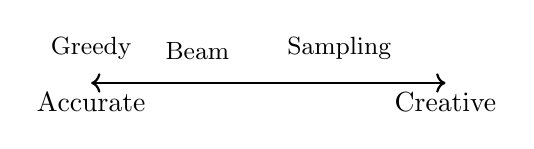
\begin{tikzpicture}[scale=0.9]
        \draw[thick, <->] (0,0) -- (5,0);
        \node[below] at (0,0) {Accurate};
        \node[below] at (5,0) {Creative};

        \node[above] at (0,0.2) {\small Greedy};
        \node[above] at (1.5,0.2) {\small Beam};
        \node[above] at (3.5,0.2) {\small Sampling};
    \end{tikzpicture}
    \end{center}

    \column{0.48\textwidth}
    \textbf{Practical Guidelines:}

    \begin{tcolorbox}[colback=green!5]
    \small
    \textbf{If accuracy critical:}\\
    Greedy or Beam + low T

    \vspace{0.3em}
    \textbf{If creativity needed:}\\
    Sampling + higher T

    \vspace{0.3em}
    \textbf{If unsure:}\\
    T=0.7, p=0.9 (good default)
    \end{tcolorbox}

    \vspace{0.5em}

    \textbf{Remember:}

    \begin{itemize}
        \item No universal best method
        \item Task determines strategy
        \item Always test and iterate
        \item User feedback is gold
    \end{itemize}
    \end{columns}
\end{frame}

% Slide 29: The Decoding Spectrum
\begin{frame}{The Complete Decoding Spectrum}
    \begin{center}
    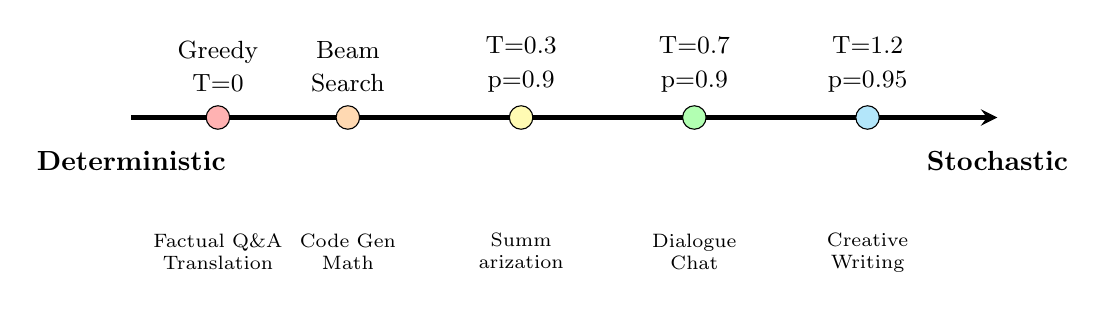
\begin{tikzpicture}[scale=1.1]
        % Main spectrum
        \draw[ultra thick, ->, >=stealth] (0,0) -- (10,0);

        % Labels
        \node[below=0.3cm] at (0,0) {\textbf{Deterministic}};
        \node[below=0.3cm] at (10,0) {\textbf{Stochastic}};

        % Methods
        \node[draw, circle, fill=red!30, inner sep=3pt] (greedy) at (1,0) {};
        \node[above=0.2cm, text width=1.5cm, align=center] at (greedy) {\small Greedy\\T=0};

        \node[draw, circle, fill=orange!30, inner sep=3pt] (beam) at (2.5,0) {};
        \node[above=0.2cm, text width=1.5cm, align=center] at (beam) {\small Beam\\Search};

        \node[draw, circle, fill=yellow!30, inner sep=3pt] (lowt) at (4.5,0) {};
        \node[above=0.2cm, text width=1.5cm, align=center] at (lowt) {\small T=0.3\\p=0.9};

        \node[draw, circle, fill=green!30, inner sep=3pt] (med) at (6.5,0) {};
        \node[above=0.2cm, text width=1.5cm, align=center] at (med) {\small T=0.7\\p=0.9};

        \node[draw, circle, fill=cyan!30, inner sep=3pt] (high) at (8.5,0) {};
        \node[above=0.2cm, text width=1.5cm, align=center] at (high) {\small T=1.2\\p=0.95};

        % Use cases below
        \node[below=0.8cm, text width=2cm, align=center, font=\scriptsize] at (1,-0.5) {Factual Q\&A\\Translation};
        \node[below=0.8cm, text width=2cm, align=center, font=\scriptsize] at (2.5,-0.5) {Code Gen\\Math};
        \node[below=0.8cm, text width=2cm, align=center, font=\scriptsize] at (4.5,-0.5) {Summ\\arization};
        \node[below=0.8cm, text width=2cm, align=center, font=\scriptsize] at (6.5,-0.5) {Dialogue\\Chat};
        \node[below=0.8cm, text width=2cm, align=center, font=\scriptsize] at (8.5,-0.5) {Creative\\Writing};
    \end{tikzpicture}
    \end{center}

    \vspace{1em}

    \begin{tcolorbox}[colback=purple!10]
    \centering
    \textbf{Your Task Determines Your Position on This Spectrum}
    \end{tcolorbox}
\end{frame}

% Slide 30: Decision Flowchart
\begin{frame}{Quick Decision Guide}
    \begin{center}
    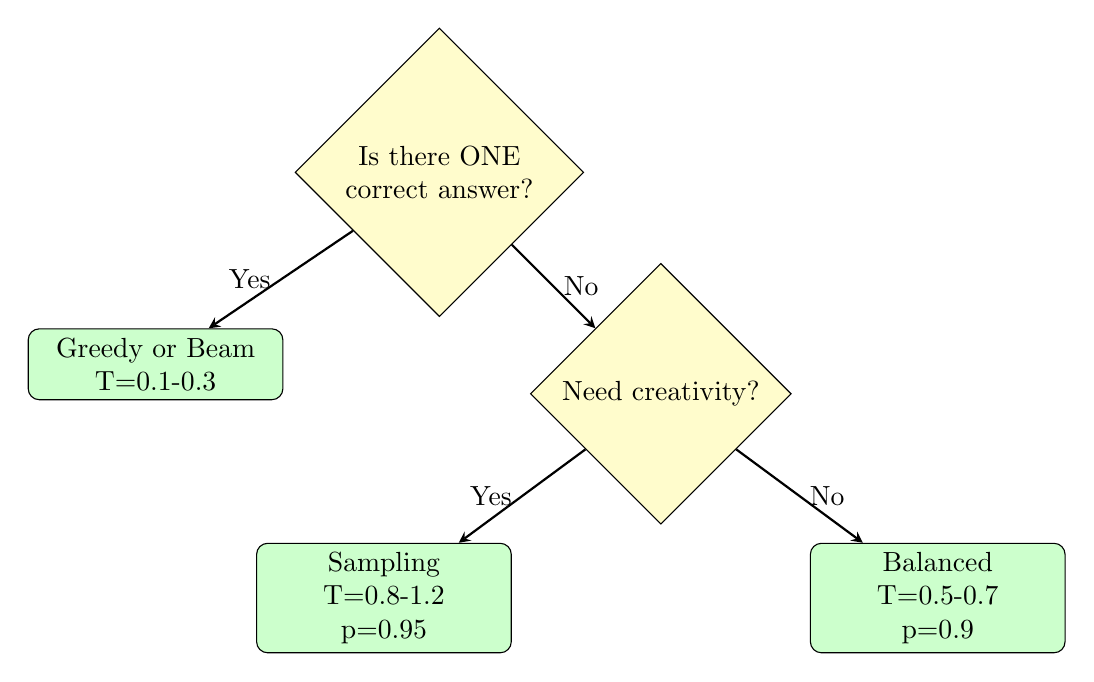
\begin{tikzpicture}[
        node distance=1.5cm,
        decision/.style={diamond, draw, fill=yellow!20, text width=3cm, text centered, inner sep=0pt},
        result/.style={rectangle, draw, fill=green!20, text width=3cm, text centered, rounded corners},
        arrow/.style={thick,->,>=stealth}
    ]
        % Start
        \node[decision] (task) {Is there ONE correct answer?};

        % Yes branch
        \node[result, below left=of task] (greedy) {Greedy or Beam\\T=0.1-0.3};

        % No branch
        \node[decision, below right=of task] (creative) {Need creativity?};

        % Creative yes
        \node[result, below left=of creative] (sample) {Sampling\\T=0.8-1.2\\p=0.95};

        % Creative no
        \node[result, below right=of creative] (balanced) {Balanced\\T=0.5-0.7\\p=0.9};

        % Arrows
        \draw[arrow] (task) -- node[left] {Yes} (greedy);
        \draw[arrow] (task) -- node[right] {No} (creative);
        \draw[arrow] (creative) -- node[left] {Yes} (sample);
        \draw[arrow] (creative) -- node[right] {No} (balanced);
    \end{tikzpicture}
    \end{center}

    \vspace{0.5em}

    \colorbox{orange!10}{\parbox{0.9\textwidth}{
    \centering\small
    \textbf{Remember:} These are starting points. Always test and adjust!
    }}
\end{frame}

% Slide 31: Looking Ahead
\begin{frame}{Next Week: Fine-Tuning \& Prompt Engineering}
    \begin{columns}
    \column{0.48\textwidth}
    \textbf{What We Learned:}

    \begin{itemize}
        \item How to decode probabilities
        \item Trade-off: accuracy vs creativity
        \item Multiple strategies available
        \item Task determines best approach
    \end{itemize}

    \vspace{0.5em}

    \textbf{Questions to Ponder:}

    \begin{enumerate}
        \item Can you combine beam + sampling?
        \item How to auto-tune parameters?
        \item What about constrained decoding?
    \end{enumerate}

    \column{0.48\textwidth}
    \textbf{Week 10 Preview:}

    \begin{itemize}
        \item Fine-tuning pre-trained models
        \item Prompt engineering techniques
        \item Few-shot learning
        \item Adapting models to your task
    \end{itemize}

    \vspace{0.5em}

    \textbf{Connection:}

    Decoding controls HOW the model generates text.\\
    Fine-tuning controls WHAT the model knows.\\
    Together: powerful customization!
    \end{columns}

    \vspace{1em}

    \begin{center}
    \textbf{Lab:} Implement all decoding strategies and compare!
    \end{center}
\end{frame}

% Technical Appendix

% Appendix A: Mathematical Formulations
\begin{frame}{Appendix A: Mathematical Formulations}
    \textbf{Temperature Scaling:}

    \begin{equation}
    P_T(w_i \given w_{<i}) = \frac{\exp(z_i / T)}{\sum_{j=1}^{V} \exp(z_j / T)}
    \end{equation}

    where $z_i$ = logit for word $i$, $T$ = temperature, $V$ = vocabulary size

    \vspace{0.5em}

    \textbf{Top-k Sampling:}

    \begin{equation}
    V_k = \{w_1, w_2, \ldots, w_k\} \text{ where } P(w_i) \geq P(w_j) \text{ for } i \leq k < j
    \end{equation}

    Sample from renormalized distribution over $V_k$ only

    \vspace{0.5em}

    \textbf{Top-p (Nucleus) Sampling:}

    \begin{equation}
    V_p = \min \left\{ V' : \sum_{w \in V'} P(w) \geq p \right\}
    \end{equation}

    \vspace{0.5em}

    \textbf{Beam Search Scoring:}

    \begin{equation}
    \text{score}(w_{1:t}) = \sum_{i=1}^{t} \log P(w_i \given w_{<i})
    \end{equation}

    With length normalization:

    \begin{equation}
    \text{score}(w_{1:t}) = \frac{1}{t^\alpha} \sum_{i=1}^{t} \log P(w_i \given w_{<i})
    \end{equation}

    where $\alpha \in [0.6, 0.7]$
\end{frame}

% Appendix B: Implementation Pseudocode
\begin{frame}[fragile]{Appendix B: Implementation Pseudocode}
    \textbf{Temperature Sampling:}

\begin{lstlisting}[language=Python, basicstyle=\small]
def sample_with_temperature(logits, T):
    # Scale logits by temperature
    scaled = logits / T
    # Apply softmax
    probs = softmax(scaled)
    # Sample from distribution
    return sample(probs)
\end{lstlisting}

    \vspace{0.5em}

    \textbf{Top-p Sampling:}

\begin{lstlisting}[language=Python, basicstyle=\small]
def top_p_sampling(logits, p):
    # Sort probabilities descending
    probs = softmax(logits)
    sorted_probs, indices = sort(probs, descending=True)
    # Find cutoff
    cumsum = cumulative_sum(sorted_probs)
    cutoff = argmax(cumsum >= p) + 1
    # Keep only nucleus
    nucleus_probs = sorted_probs[:cutoff]
    nucleus_indices = indices[:cutoff]
    # Renormalize and sample
    nucleus_probs = nucleus_probs / sum(nucleus_probs)
    sampled_idx = sample(nucleus_probs)
    return nucleus_indices[sampled_idx]
\end{lstlisting}
\end{frame}

% Appendix C: Performance Benchmarks
\begin{frame}{Appendix C: Performance Benchmarks}
    \textbf{Translation Task (WMT14 EN-DE):}

    \begin{center}
    \begin{tabular}{lcccc}
    \textbf{Method} & \textbf{BLEU} & \textbf{Speed} & \textbf{Diversity} & \textbf{Repetition} \\
    \hline
    Greedy & 26.5 & 100\% & 0.21 & 15\% \\
    Beam-4 & \textbf{28.2} & 25\% & 0.24 & 12\% \\
    T=0.5, p=0.9 & 26.8 & 80\% & 0.35 & 8\% \\
    T=1.0, p=0.9 & 25.1 & 80\% & 0.52 & 5\% \\
    \end{tabular}
    \end{center}

    \vspace{0.5em}

    \textbf{Story Generation (WritingPrompts):}

    \begin{center}
    \begin{tabular}{lcccc}
    \textbf{Method} & \textbf{Coherence} & \textbf{Creativity} & \textbf{Human Pref} & \textbf{Distinct-2} \\
    \hline
    Greedy & 4.2/5 & 2.1/5 & 15\% & 0.18 \\
    Beam-5 & 4.0/5 & 2.5/5 & 20\% & 0.22 \\
    T=0.8, p=0.9 & 3.8/5 & 3.9/5 & 35\% & 0.51 \\
    T=1.0, p=0.95 & 3.5/5 & \textbf{4.3/5} & \textbf{40\%} & \textbf{0.62} \\
    \end{tabular}
    \end{center}

    \vspace{0.5em}

    \textbf{Key Observations:}
    \begin{itemize}
        \item Beam wins on translation (objective metrics)
        \item Sampling wins on creative writing (human preference)
        \item Trade-off between coherence and diversity is real
        \item No single best method across tasks
    \end{itemize}
\end{frame}

\end{document}
